\documentclass{article}
\usepackage[utf8]{inputenc}
\usepackage{ wasysym }
\usepackage{ upgreek }
\usepackage{ amssymb }
\usepackage[margin=1.2in]{geometry}
\usepackage[pdftex]{graphicx}
\usepackage{blindtext}
\setlength{\emergencystretch}{3em}
\usepackage{fancyhdr}
\pagestyle{fancy}
\lhead{IMMC18624740}
\rhead{}


\title{Demographic Transition in Three Decades Ahead}
\author{IMMC18624740}
\date{November 2017}

\begin{document}

\maketitle

\section{Abstract}
\paragraph{}

\section{Problem Restatement}
\paragraph{}

\section{Assumptions}
\paragraph{$\checked$ There are no huge medical breakthroughs in the following thirty years. \\
Justification: With a relatively small probability of developing reinvigorated medical technology or practices which may affect the fertility rate and mortality rate, it can be seen as a negligible factor. }
\paragraph{$\checked$ Major population-crippling disasters will not happen during the time period of our model. \\
Justification: Major population crippling disasters, such as wars and natural disasters, are likely to affect population significantly. We can't account for this since the probability of these events happening are scant.}
\paragraph{$\checked$ Emigration from urban areas can be ignored. \\
Justification: Developing rapidly, more and more villagers prefer to move to urban areas, and there will be only a few urbanites who are willing to move out, which is neglectable. }
\paragraph{$\checked$ The emigrants' change of population per year may be considered as several points in a cubic function. \\
Justification: Some people are moving out of their home country, and the number of the population changes every year. By fitting the function, we find the emigrants' change of population per year can be written in form of a cubic function. }
\paragraph{$\checked$ The large movement of people during special periods of time is not considered in our model. \\
Justification: For instance, during the Spring Festival Travel Rush, temporary migration is going to change regional population trends dramatically, and is too complex to consider.}
\paragraph{$\checked$ Tourism is an unpredictable and unimportant value, thus is neglected in our model. \\
Justification: It is unable to have the accurate data of volatile and impermanent value, and there is no use to add it in our model. }
\paragraph{$\checked$ The death rates of urban area and rural area are the same. \\
Justification: The differences of death rates between urban area and rural area has few influence in our further model which is about urbanization, so to neglect the differences is a workable assumption. }
\paragraph{$\checked$ Young adults' behaviors and attitudes does not change in the next thirty years. \\
Justification: In predicting the satellite city construction, we may assume young adults act and think as same as today's majority group of young adults, in order to distribute arrange people of different ages to different regions. }
\paragraph{$\checked$ The Two-child policy is not considered in this model. \\
Justification: The Two-child policy in China came out in 2016, and there isn't data on the population changes that year. We couldn't get a good result to base off of, so we excluded the small fertility increase due to this policy.}
\paragraph{$\checked$ Developed regions have the same amount of resources, and the undeveloped regions have had the same value. \\
Justification: The amount of resources plays an important role in evaluating the city's carrying capacity, so it is necessary to assume with the same amount of resources. }


\section{Designing The Mathematical Model}
\paragraph{We have designed a population model, in order to develop and examine a further model about the effects on population of urbanization.}

\subsection{Population Model}
\paragraph{Based on One Child Policy, we designed a population model, which is able to show the population of each year, after the publishing of One Child Policy in 1979. It helps with understanding the complicated process of population growth. \\
In general, a population model can be written in form of a function, as shown below.}
\paragraph{$$P=P_0 +B-D-A$$}
\paragraph{where, \\
$\bell$ $P$ is the population of the country\\
$\bell$ $P_0$ is the population of the first year \\
$\bell$ $B$ is the number of new born babies in that year\\
$\bell$ $D$ is the number of dead in that year\\
$\bell$ $A$ is the number of emigrants who are no longer citizens}
\paragraph{To get a more accurate number of population, we choose to add several variables, such as mortality, fertility, and life expectancy. These variables play important role in the One Child Model, and after integration, we get the following function: }
\paragraph{$$P(t)=P(t-\upalpha)\prod_{i=t-\upalpha}^t \left(1-\frac{1}{1000}m(i)+s_rf(i)\frac{1}{E(i-\upbeta)}\right)-\sum_{i=t-\upalpha}^t A(t)$$}
\paragraph{where \\
$\bell$ $P$ is the population of the country as a function of time \\
$\bell$ $t$ is the number of the year \\
$\bell$ $\upalpha$ is the start of the calculation (from 1979, for mainland China) \\
$\bell$ $m$ is the mortality rate per 1000 people \\
$\bell$ $s_r$ is the sex ratio \\
$\bell$ $f$ is the fertility rate per women \\
$\bell$ $E$ is the life expectancy \\
$\bell$ $\upbeta$ is the average age of birth giving mothers (suppose it is 26) \\
$\bell$ $A$ is the emigrant amount \\}
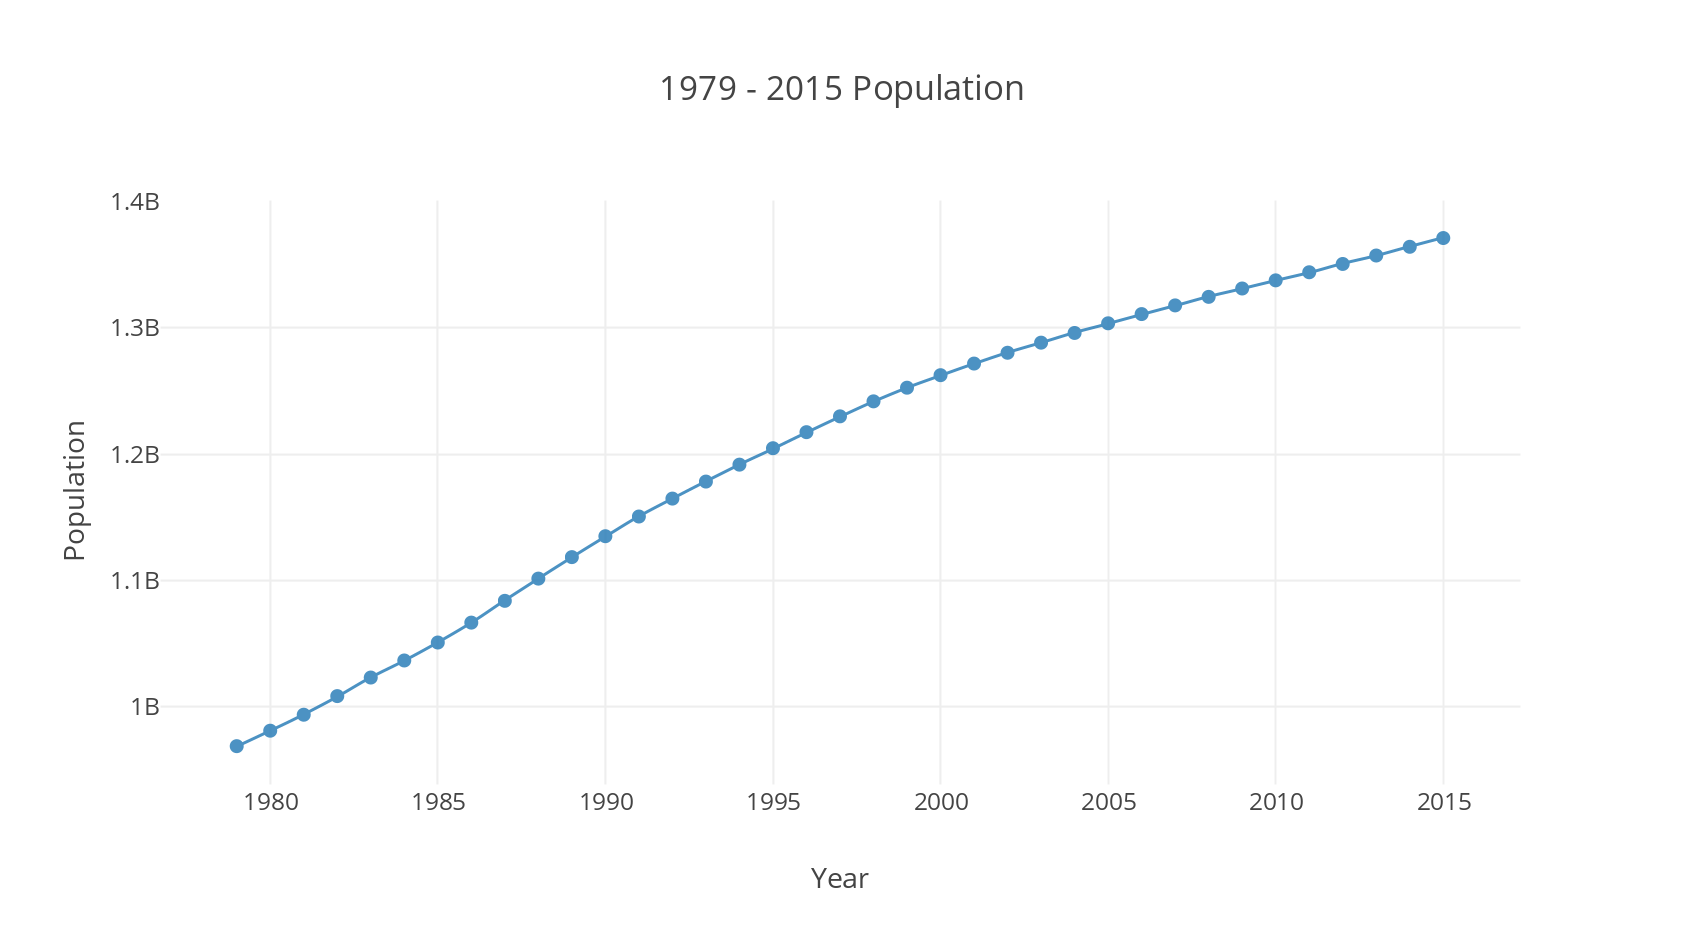
\includegraphics{Population15.png}
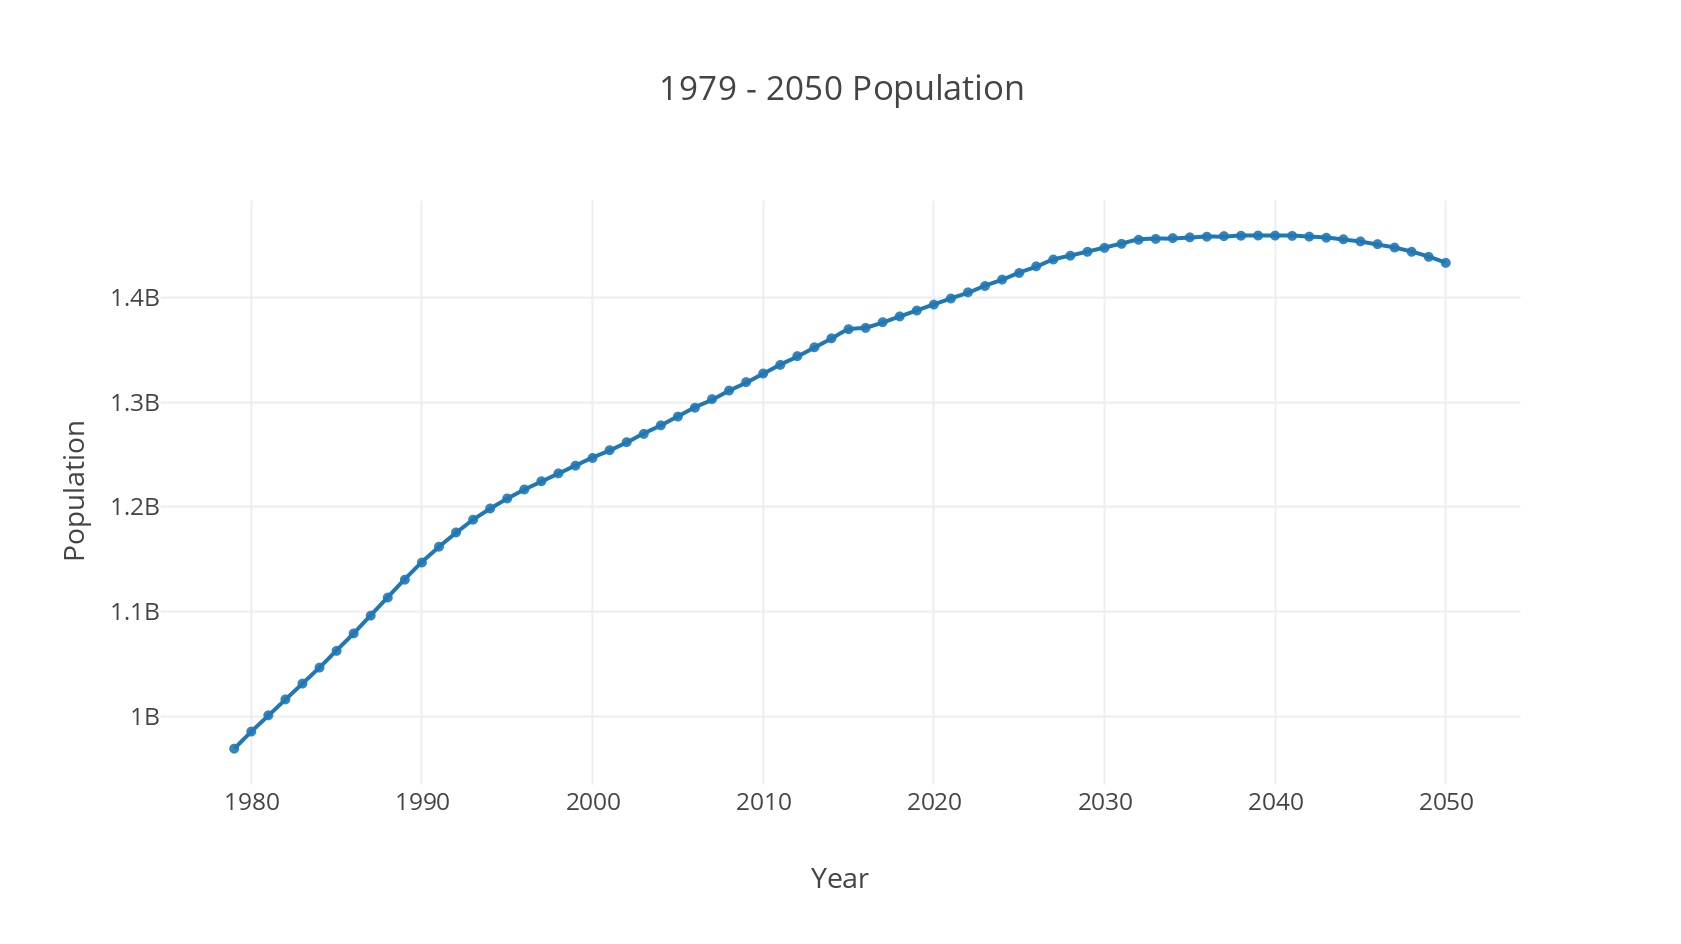
\includegraphics{Population50.png}

\subsection{Sensitivity Analysis}
\paragraph{Our model has covered several main factors; however, there are still a few uncontrollable factors that are likely to effect the solution of our model. In order to handle uncertainty, we have to analyze the sensitivity of our model, based on sensitive comprehensive evaluation result. \\
To analyze the sensitivity, we ran our model with different sets of probabilities, and it is proved that our model is very sensitive. We chose m, the mortality rate, and f, the fertility rate, as two changing variables, trying to simulate situations of small changes. \\
We tested our model with a population crippling disaster, an epidemic, to have a sudden mortality rate change. By having F-Test, the One Child Model indicates that, with a relatively high p-value, it is likely and possible, and our initial model of One Child Model is capable of adapting random events and different circumstances, effectively. \\
Further details can be found in Appendix-8.1}

\subsection{Strengths of Our Model}
\paragraph{1. We used a combination of past data and regression models to develop our population estimate, which is very accurate. Our model only uses a starting population, which is very easy to come by.\\ 
2.We used statistics from authoritative sites, for example: National Bureau of statistics of China, The World Bank DATA, UNdata, etc, so our data used is reliable. \\
3. Our model was based on our own inspirations and ideas, and fully authentic. Thus, no copyright issues are involved. \\
4. Our model can be applied to both estimating national population and regional population, giving the model a wider usage. \\ }

\subsection{Weakness of Our Model}
\paragraph{1. The model cannot calculate population growth prior to 1979 or after thirty years from now. \\
2. For the sake of simplifying our model, some outlier data points were eliminated from the regression models, thus resulting in some variations between our model and the real data. Some events are hard to quantify, so we left these out of the picture. }

\section{Models of Urbanization}
\paragraph{Based on our One Child Model, we developed an Urbanization-Dependent Model, in sake of predicting population of urban area. As we know, the Logistic Model fits in population models. So we compared these two model's maximum and created an Artificial Intelligence of predicting when the city will reach its carrying capacity.}

\subsection{Urbanization-Dependent Model}
\paragraph{Since we have derived the function of population of a country(see 4.1-Population Model), we may use a similar function when evaluating a city's population. However, it differs; during the process of urbanization, people move from rural area to urban area. So, we decide to add a variable, $U$, into the function, shown by, }
\paragraph{$$P(t)=P(t-\upalpha)\prod_{i=t-\upalpha}^t \left(1-\frac{1}{1000}m(i)+s_rf(i)\frac{1}{E(i-\upbeta)}\right)-\sum_{i=t-\upalpha}^t A(t)+U(t)$$}
\paragraph{where, \\
$\bell$ $U$ is the population change between urban area and rural area as a function of time \\
(All the other symbols remain the same definition as it is shown in 4.1-Population Model) }
\paragraph{The Urbanization-Dependent Model have a great possibility to be accurate and show a clearer graph of changes in population of urban areas than other functions, since it is based on real data. However, we have to compare it to a model which is created theoretically. }

\subsection{Logistics Model}
\paragraph{According to Pierre François Verhulst's model of population growth, which indicates the proportion of the rate of reproductive and the amount of resources and the existed population. }

\paragraph{We may also write the function in form of logistic function, which is the control group of the population model, shown by, }
\paragraph{$$P(t)=\frac{K\cdot P_0\cdot e^{rt}}{K+P_0\cdot (e^{rt}-1)}$$}
\paragraph{where \\
$\bell$ $P$ is the population of a city as a function of time \\
$\bell$ $t$ is the number of the year \\
$\bell$ $K$ is the carrying capacity of the city
$\bell$ $P_0$ is the cardinality of the population of the city, when t=1979 \\
$\bell$ $e$ is a mathematical constant that is the base of natural logarithm \\
$\bell$ $r$ is the reproductive capacity, which is the product of sex ratio and the probability of females who have higher fertility(15-44) getting pregnant that year; and we calculated that the value of $r$ is a constant: 0.075}

\paragraph{The previous function represent how the population of a city changes, in consideration of the carrying capacity, sex ratio and age distribution. Therefore, we may compare and contrast two functions, which are shown in 5-Model, and compute the population of some typical cities in Mainland China, to make sure that our model about urbanization is accurate, in a certain period of time. }

\subsection{Real-World City Analysis}
\paragraph{We first analyzed the relationship between the maximum ...}

\section{Satellite City Construction}
\subsection{Overpopulation}
\paragraph{Using our model of the city of Beijing and the carrying capacity of the city, we predicted that the population of Beijing will start to approach the carrying capacity in the year 2030. To solve this population increase issue, the government of China has devised the following solutions:}
\paragraph{$\bigstar$ Limiting the number of migrants to the city \\
$\bigstar$ Creating a satellite city, Xiong'an New Area, and relocating half a million individuals to that city}

\subsubsection{Problems}
\paragraph{These solutions adopted by the government still have some problems. We analyzed the second solution, creating a satellite city, and found out that the population of Beijing will still exceed the carrying capacity, only delayed by around 12 years. Thus, we will propose our own solution.}
\subsubsection{Data}
\subsection{Our Solution}
\paragraph{}


\section{Conclusion}

\section{Appendix}
\subsection{Variables of the One Child Model}
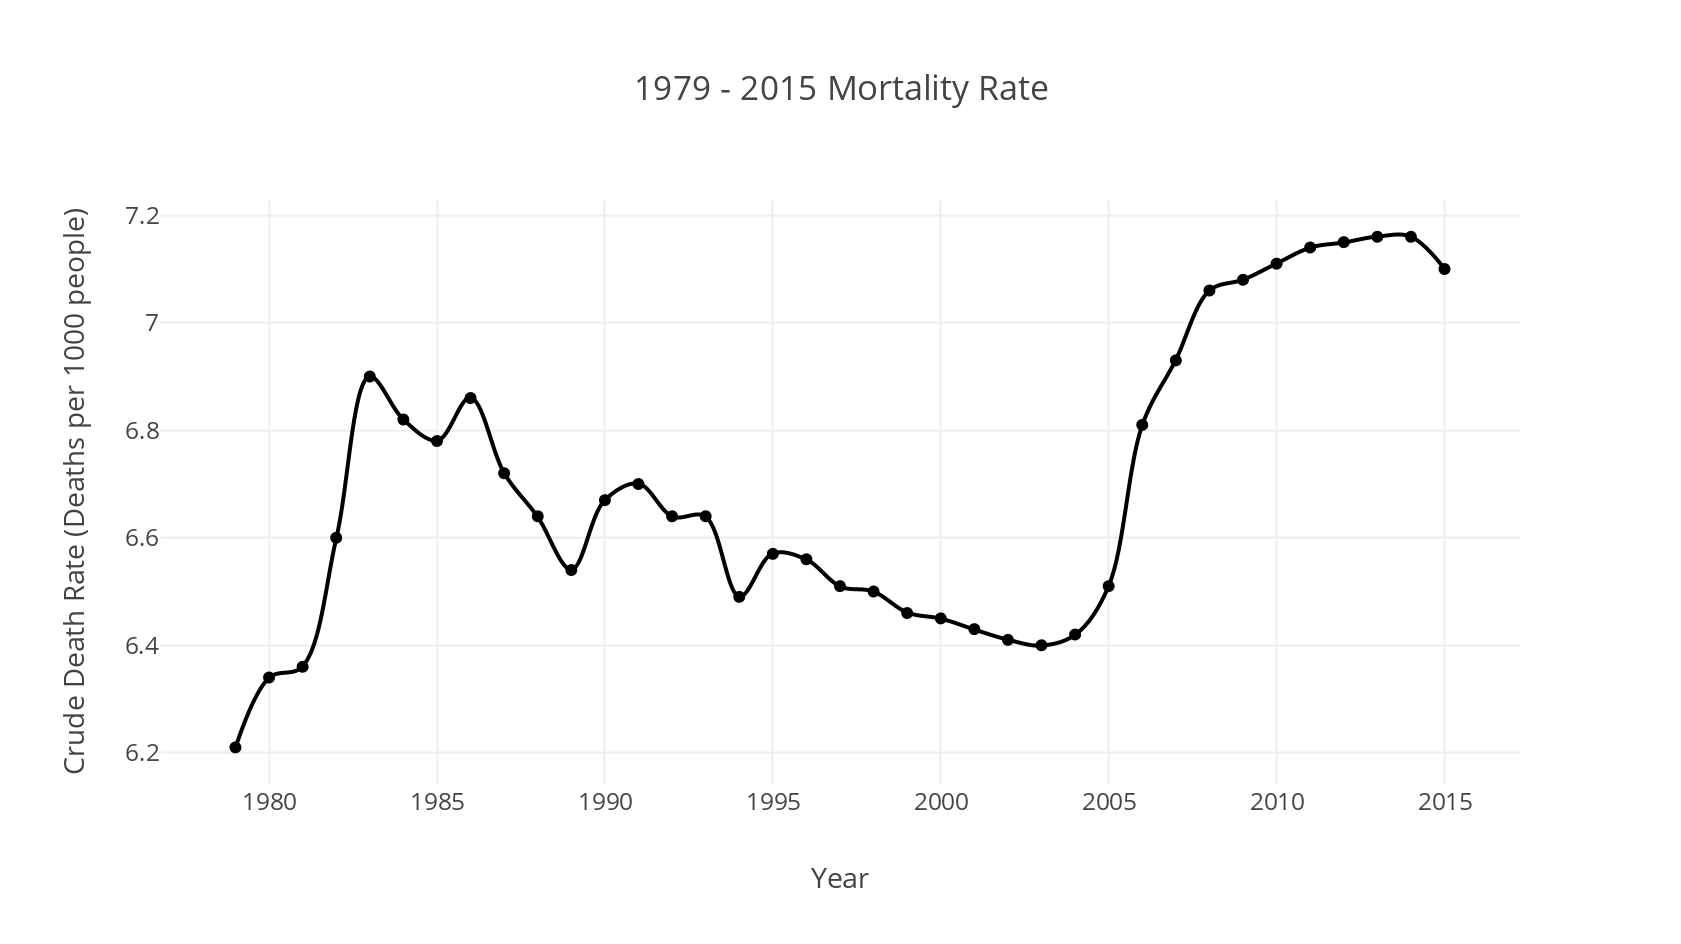
\includegraphics{MortalityRate.png}
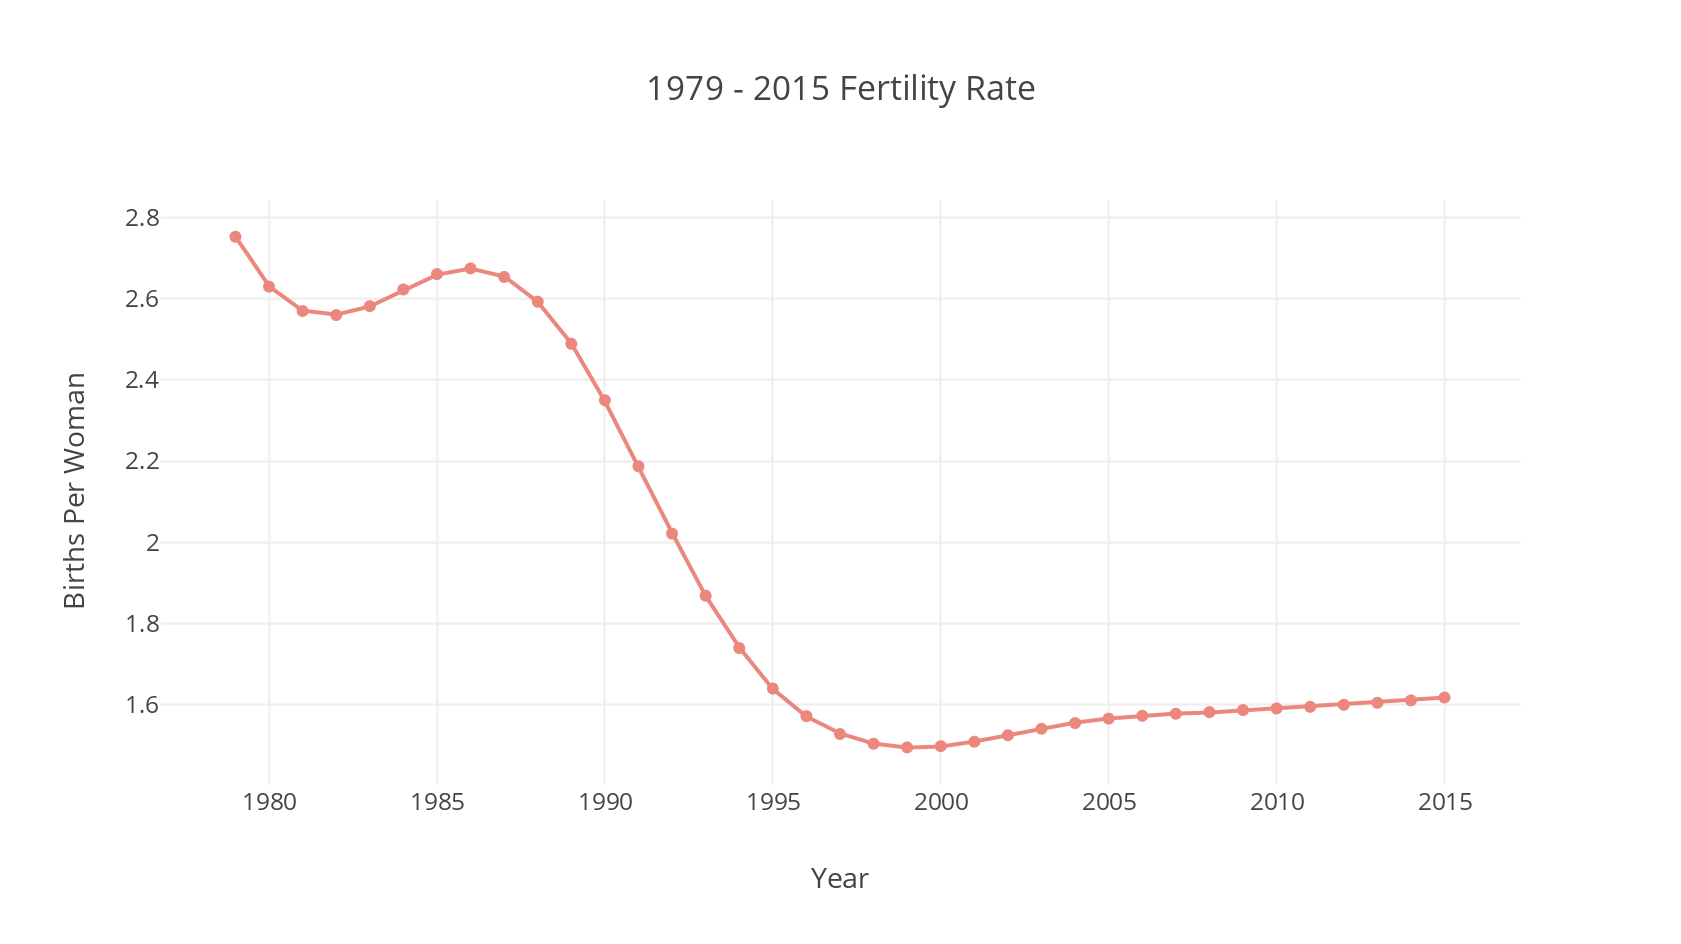
\includegraphics{FertilityRate.png}
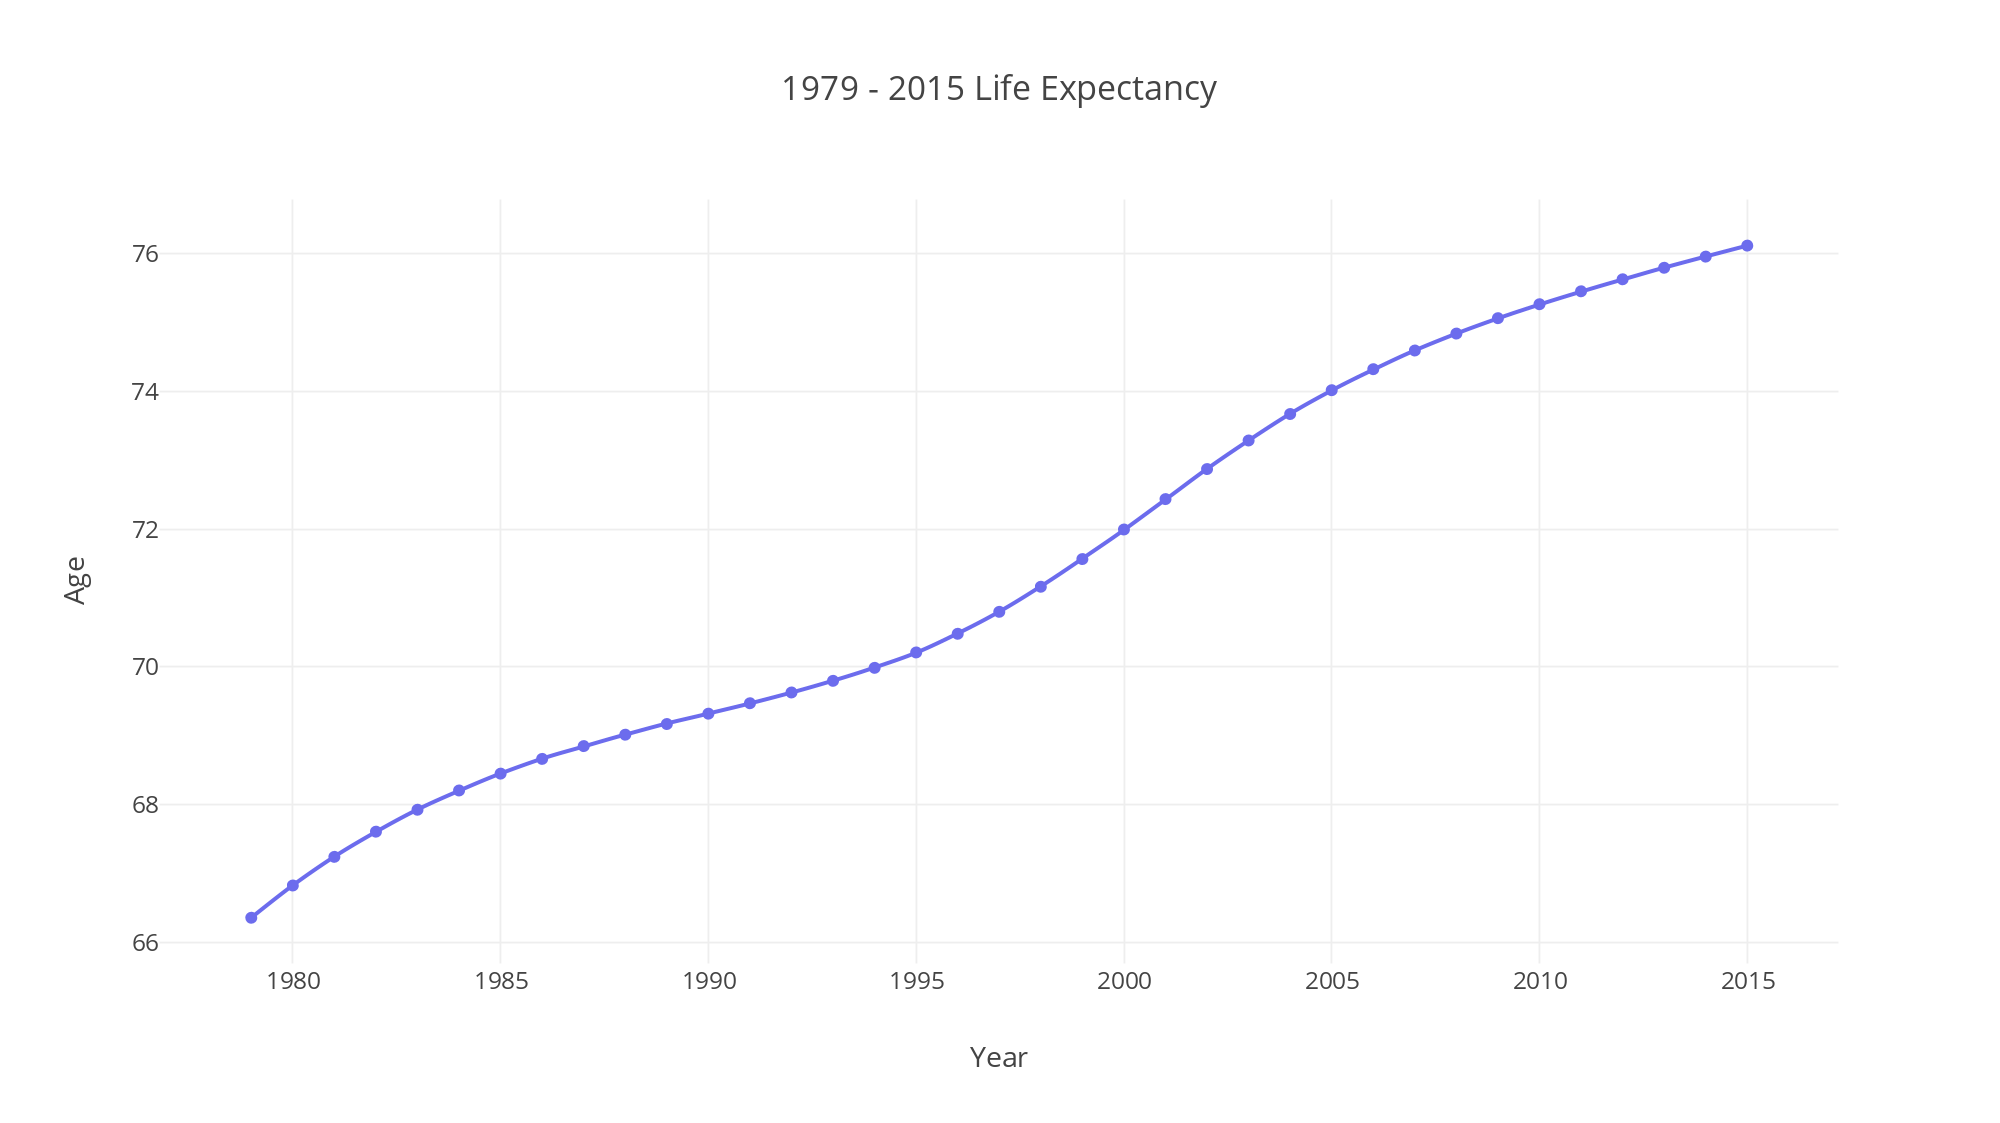
\includegraphics{LifeExpectancy.png}

\subsection{F-Test of the One Child Model}
\paragraph{FonewayResult(statistic=0.0051791669112102113, pvalue=0.94282816249558166)}


\end{document}